% Laid out like a NASA Technical Memorandum (report page, abstract, numbered
% sections, formal references), but published as independent team work: we may
% not use the NASA insignia or call this a NASA publication (Space Apps rules).
% Every number in this file comes from submission/evidence/*.json or from
% report/figures/make_figures.py; rebuild with ./reproduce_report.sh.
\documentclass[11pt,a4paper]{article}
\usepackage{fontspec}
\setmainfont{TeX Gyre Termes}
\usepackage[margin=2.3cm]{geometry}
\usepackage{graphicx,booktabs,siunitx,hyperref,xcolor,caption}
\usepackage[style=authoryear,backend=biber,maxcitenames=2,uniquelist=false]{biblatex}
\addbibresource{references.bib}
\hypersetup{colorlinks,linkcolor=blue!50!black,citecolor=blue!50!black,urlcolor=blue!50!black}
\captionsetup{font=small}

\title{HIPPARCHUS: Validated Multi-Epoch Comparison of SPHEREx Imaging\\
\large Independent Technical Report AITHENOVA-TR-2026-01}
% Single-member team.
\author{Evangelos Tampachaniotis (Team AITHENOVA) \\ NASA Space Apps Challenge 2026, Athens \\ \small Challenge: Planet X and SPHEREx}
\date{15 November 2026}

\begin{document}
\maketitle
\noindent\fbox{\parbox{\dimexpr\linewidth-2\fboxsep}{\small
This is an independent report by Team AITHENOVA, written during the NASA Space Apps Challenge 2026.
It is not a NASA publication and has not been reviewed or endorsed by NASA. SPHEREx data are provided by
NASA/IPAC IRSA.}}

\begin{abstract}
SPHEREx images the entire sky repeatedly, so any star can in principle be compared across epochs. Doing this
naively gives false results: the linear variable filters put the same star at a different wavelength in every
visit, bright stars saturate, and zodiacal light changes with the season. HIPPARCHUS is an open tool that finds
every SPHEREx exposure of a position in the NASA/IPAC IRSA archive, checks each one, and compares only pairs that
are scientifically compatible, refusing the others with a stated reason. On real DR1 and QR3 data it finds
8 valid comparisons out of 1540 possible pairs for RW~Aurigae in detector~1. In all of them the star is brighter in the later
epoch, by up to a factor of $2.56$ over 371 days ($175\sigma$ formal), while a control star in the same images stays
constant within $2.2\sigma$. For Barnard's Star it rejects all 58 epochs as saturated and refuses to compare. For the faint
brown dwarf WISE~0855$-$0714 it finds 27 valid pairs and no significant change, with a scatter of significances
(0.83) that shows the error model is not underestimated. All inputs, checksums, settings and outputs are recorded.
\end{abstract}

\section{Introduction}
The Planet X and SPHEREx challenge asks how SPHEREx data can reveal things that change or move in the sky.
SPHEREx \parencite{dore2014} observes every point of the sky several times a year in 102 spectral channels between
about 0.75 and \SI{5}{\micro\meter}, using linear variable filters (LVFs): the wavelength seen by a pixel depends on
where it lies on the detector. A star is therefore observed at a different wavelength in each visit. Comparing two
raw images of the same star and calling the difference ``variability'' is wrong unless the wavelengths agree.

HIPPARCHUS (named after the astronomer who found that stars change and move by comparing his catalogue with older
ones) is built around one idea: \emph{a comparison is only reported when it is valid, and otherwise refused with a
reason a person can check}. Refusal is a result, not a failure.

\section{Data}
All images come from the IRSA image search service (IVOA SIA~v2, \url{https://irsa.ipac.caltech.edu/SIA}) for two
collections: SPHEREx DR1 spectral images \parencite{irsa_dr1} and Quick Release QR3 \parencite{irsa_qr3}. When an
exposure is in both, the DR1 version is used. Only \texttt{science} products are kept. For each exposure we request a
$0.05^\circ$ server-side cutout (about $29\times29$ pixels of $6.15''$) and store it with its SHA-256 checksum; the
checksum is verified every time a cached file is reused. Each cutout contains the calibrated image (MJy\,sr$^{-1}$),
the pipeline flags, the variance, the zodiacal-light model and a spectral WCS lookup table.

Table~\ref{tab:targets} lists the three demonstration targets. Their positions are approximate priors used only to
centre the cutouts; the star is measured in the images. The main CDS servers were offline after a cybersecurity
incident \parencite{cds_incident2026} and the ESA Gaia archive did not answer, so the presets were later checked against
SIMBAD \parencite{simbad2000} and Gaia DR3 \parencite{gaiadr3} through the mirrors CDS recommends (Section~\ref{sec:val}).

\begin{table}[h]\centering\small
\caption{Targets and archive coverage (queries of 15 November 2026, all \emph{live}).}\label{tab:targets}
\begin{tabular}{lcclrrr}\toprule
Target & RA ($^\circ$) & Dec ($^\circ$) & Detector & Epochs & Usable & Span \\\midrule
RW Aurigae & 76.956 & $+30.401$ & D1 & 56 & 18 & 2025-09-01 -- 2026-09-09\\
Barnard's Star & 269.4463 & $+4.7667$ & D6 & 58 & 0 & 2025-08-15 -- 2026-08-20\\
WISE 0855$-$0714 & 133.7600 & $-7.2424$ & D6 & 45 & 37 & 2025-05-05 -- 2026-05-11\\\bottomrule
\end{tabular}
\end{table}

\section{Method}
\paragraph{Per-epoch checks.} For each cutout we (1) subtract the pipeline's zodiacal-light model, since zodiacal
light changes with the season; (2) locate the target with the celestial WCS (TAN-SIP); (3) read the wavelength and
channel width \emph{at the target pixel} from the spectral lookup WCS; and (4) reject the epoch if the target lies
within the aperture radius of the cutout edge, if any pixel within $r=2$\,px carries a rejecting flag (OVERFLOW,
NONLINEAR, TRANSIENT, SUR\_ERROR, PERSIST, BLOOM, GHOST, HOT, and others; 18 planes in total, read by name from each
file's own FLAGS header), if values are missing, or if the variance is not positive. SOURCE is not a rejecting flag,
since the target is itself a source; DICHROIC and PHANMISS are reported as warnings.

\paragraph{Pair compatibility.} Two epochs are compared only if both are usable, come from the same detector, and
the target's wavelengths differ by at most half a channel width. Pairs taken less than 0.5 days apart are treated as
null tests of the noise.

\paragraph{Comparison.} The later image, its variance and its flag mask are reprojected onto the earlier epoch's
pixel grid (\texttt{reproject}, bilinear). Flux is the sum inside $r=2$\,px minus the median sky in a 4--7\,px
annulus; its uncertainty combines the pixel variances and the error of the sky level. A change is called significant
at $|\Delta F|/\sigma_{\Delta F}\ge5$. We also report the flux ratio, a per-pixel significance map, and the shift of the
light-weighted centroid in arcseconds. As a check of calibration, the brightest clean local peak at least 9\,px from
the target is measured the same way in the same two images (\emph{control star}).

\section{Validation}\label{sec:val}
\begin{itemize}\setlength\itemsep{1pt}
\item \textbf{Unit tests} (35, \texttt{pytest}) run on real SPHEREx cutouts committed as fixtures, with their source
URL and checksum recorded. They cover cache integrity, flag decoding from headers, refusal of files that lack a
required extension, targets near RA~$0^\circ$, wavelength at the target, refusal of wavelength mismatches and flagged
epochs, the classification of same-visit pairs, a self-comparison that must show no change ($|\sigma|<0.5$ after
reprojection), the control-star check, the evidence graph, proper-motion propagation and catalogue matching, and that a partial archive answer never replaces a
complete saved listing.
\item \textbf{Control stars.} For the six RW~Aur pairs with a control star, its ratio lies between 0.86 and 1.07 and
its significance between $-2.2\sigma$ and $+0.7\sigma$ (Table~\ref{tab:rw}).
\item \textbf{Error model.} For WISE~0855, where the target is barely detected (median $S/N\approx2.7$ per epoch), the
27 pair significances have a standard deviation of 0.83 and a maximum of $|1.9|\sigma$. They behave like noise, so
the formal errors are not underestimated at low flux.
\item \textbf{Null test with blank apertures.} No same-visit pairs exist for these targets, so we run the same
photometry at a grid of positions away from the target in every valid pair (positions $5$\,px apart, clear of masked
pixels). Sky and ordinary stars should not change, so with correct errors the significances spread with standard
deviation 1. We find 1.08 for WISE~0855 ($n=55$), 0.55 for RW~Aur ($n=38$) and 0.91 overall ($n=93$), with no value
beyond $3\sigma$ (Figure~\ref{fig:val}, left). The errors are therefore right or conservative. For RW~Aur they are
too large by about a factor of two; Section~\ref{sec:rob} shows this is not caused by the reprojection.
\item \textbf{Injection-recovery (SIMULATED).} We add artificial Gaussian stars (FWHM from the image header) to the
later epoch at the same blank positions, with known $S/N$ inside the aperture, and rerun the comparison. These
sources are simulated, are kept in a separate section of \texttt{validation.json}, and are never mixed with real
measurements. The method recovers 44\% at $S/N=5$, 87\% at 6 and 99\% at 7 (Figure~\ref{fig:val}, right), as
expected for a $5\sigma$ threshold; nothing is recovered below $S/N=3$. The photon noise of the injected star is not
added, which makes bright injections slightly easier than real ones.
\item \textbf{Evidence graph.} Each result is linked to its epochs, cutouts (SHA-256), observations, archive queries
(SHA-256 of the raw answer) and the dataset DOI. For all three targets the graph has no broken links and no result
without a DOI (\texttt{submission/evidence/graph\_*.json}); a test checks that a broken link is detected.
\item \textbf{Catalogue match.} SIMBAD (CfA Harvard mirror) and Gaia DR3 (IRSA copy) were queried on
15~November~2026; both positions were moved to epoch 2026.0 with their proper motions.
The answers and their SHA-256 are kept in \texttt{catalog\_match.json}. All three presets fall on the right object: RW~Aur is
$2.1''$ (0.34~px) from SIMBAD, Barnard's Star $5.4''$ (0.88~px; it moves $10''$ per year), WISE~0855 $1.1''$
(0.19~px). The match also shows what lies inside our $12.3''$ aperture: for RW~Aur both components of the binary
(Gaia $G=13.0$ and $12.2$, $1.6''$ apart) and a $G=18.8$ star; for WISE~0855, which Gaia does not detect, a
$G=16.3$ field star $6.8''$ away.
\end{itemize}

\begin{figure}[h]\centering
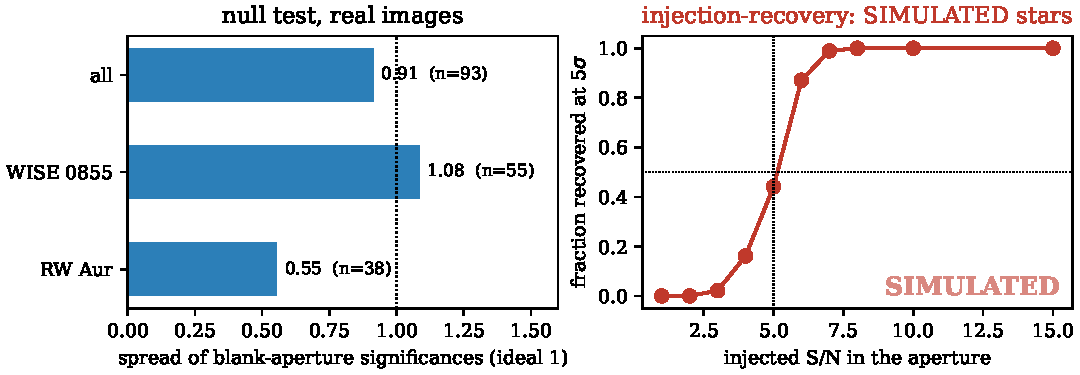
\includegraphics[width=\linewidth]{figures/validation.pdf}
\caption{Left: spread of the significance of ``change'' at blank positions in the real image pairs; 1 means correct
error bars. Right: fraction of SIMULATED injected stars recovered at $5\sigma$ against their injected $S/N$.}
\label{fig:val}
\end{figure}

\section{Results}
\paragraph{A. Valid comparison: RW Aurigae.} RW Aur is a young star with a history of deep dimming events caused by
its disk \parencite{rodriguez2013}. Of 1540 possible pairs, 1480 fail the wavelength test and 1387 involve a flagged
epoch (mostly OVERFLOW: RW Aur saturates detector~1 in 37 of 56 epochs). Eight pairs remain (Table~\ref{tab:rw}). In
all eight the star is brighter in the later epoch. The pairs chain consistently: $\times1.67$ from September 2025 to
March 2026, then $\times1.42$ to September 2026, giving $\approx\times2.4$ against $\times2.50$--$2.56$ measured directly. The
centroid moves by $<0.8''$ (an eighth of a pixel), so the light comes from the same star. Figure~\ref{fig:rw} shows the
strongest pair.

\begin{table}[h]\centering\small
\caption{All valid comparisons for RW Aur, detector D1. Ratio = later/earlier flux; control = ratio and significance
of the control star in the same images.}\label{tab:rw}
\setlength{\tabcolsep}{4pt}\footnotesize
\begin{tabular}{llrcrrlr}\toprule
Earlier & Later & $\Delta t$ (d) & $\lambda$ (\si{\micro\meter}) & Ratio & Signif. & Control & Shift ($''$)\\\midrule
2025W36\_1A\_0233\_3 & 2026W37\_1A\_0234\_3 & 371.2 & 0.763/0.770 & 2.56 & 175.1 & 0.86 ($-1.4$) & 0.59 \\
2025W36\_1A\_0233\_2 & 2026W37\_1A\_0234\_2 & 371.2 & 0.745/0.752 & 2.50 & 173.5 & 1.07 (0.7) & 0.14 \\
2026W11\_1A\_0285\_1 & 2026W37\_1A\_0234\_3 & 181.8 & 0.774/0.770 & 1.50 & 84.8 & 0.89 ($-1.1$) & 0.78 \\
2025W36\_1A\_0233\_3 & 2026W10\_2B\_0591\_4 & 187.6 & 0.763/0.757 & 1.67 & 84.4 & 0.90 ($-1.1$) & 0.48 \\
2026W10\_2B\_0591\_4 & 2026W37\_1A\_0234\_2 & 183.6 & 0.757/0.752 & 1.42 & 80.3 & 0.97 ($-2.2$) & 0.75 \\
2025W36\_1A\_0233\_2 & 2026W10\_2B\_0591\_3 & 187.6 & 0.745/0.739 & 1.62 & 80.3 & 0.95 ($-0.5$) & 0.16 \\
2025W36\_1A\_0446\_1 & 2026W11\_1A\_0285\_1 & 188.5 & 0.781/0.774 & 1.41 & 55.0 & -- & 0.32 \\
2025W36\_1A\_0606\_2 & 2026W10\_1A\_0445\_2 & 181.6 & 0.878/0.878 & 1.09 & 18.5 & -- & 0.27 \\\bottomrule
\end{tabular}
\end{table}

\begin{figure}[h]\centering
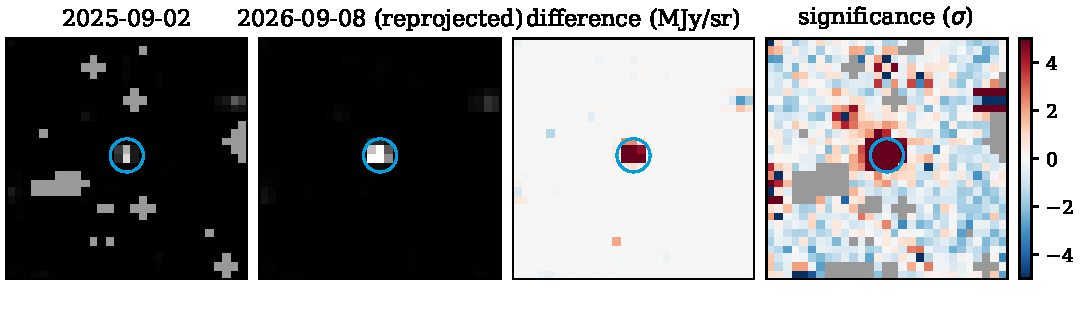
\includegraphics[width=\linewidth]{figures/rwaur_pair.pdf}
\caption{RW Aur in detector D1, 2025-09 and 2026-09, the later image reprojected onto the earlier grid; the
difference; and the per-pixel significance ($\pm5\sigma$). Grey: pixels masked by flags. Circle: photometry aperture.}
\label{fig:rw}
\end{figure}

\begin{figure}[h]\centering
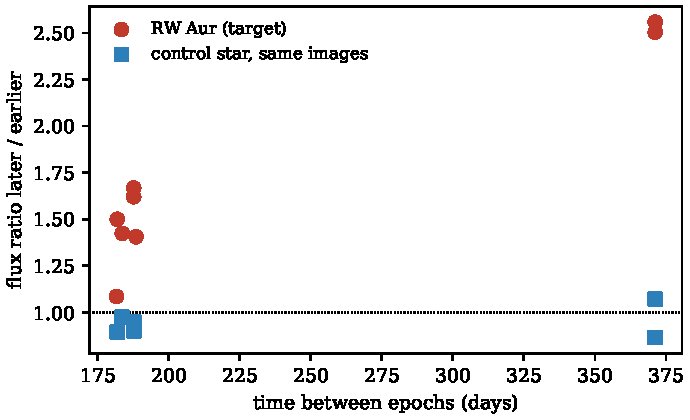
\includegraphics[width=0.48\linewidth]{figures/rwaur_ratios.pdf}\hfill
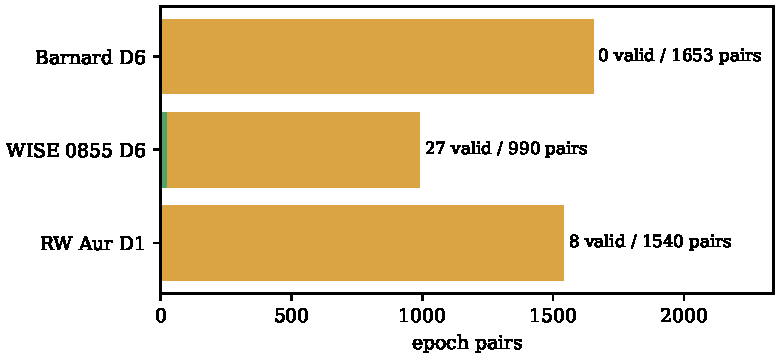
\includegraphics[width=0.48\linewidth]{figures/pair_outcomes.pdf}
\caption{Left: flux ratio of each valid RW Aur pair (red) and of its control star (blue). Right: for each target,
the fraction of all epoch pairs that pass every check.}\label{fig:ratios}
\end{figure}

\paragraph{B. Refused comparison: Barnard's Star.} Barnard's Star is far too bright for SPHEREx at
\SI{4.4}{}--\SI{5}{\micro\meter}. All 58 D6 epochs are rejected: OVERFLOW on the target in 56, TRANSIENT in 53, BLOOM in 54,
SUR\_ERROR in 45; one epoch also has missing values and variance on the target (Figure~\ref{fig:barnard}). HIPPARCHUS reports
\emph{no valid comparison} and lists these reasons. A naive difference of these images would have shown large
``changes'' caused by saturation and by the star's high proper motion, so refusing is the correct answer.

\begin{figure}[h]\centering
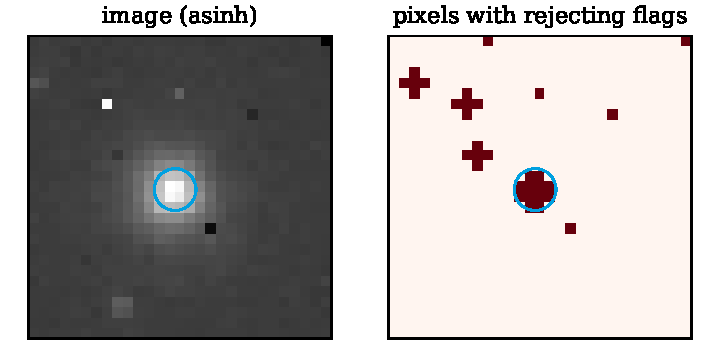
\includegraphics[width=0.55\linewidth]{figures/barnard_flags.pdf}
\caption{A rejected Barnard's Star epoch (2025W33\_2C\_0321\_1, D6) and the pixels whose flags make it unusable.}
\label{fig:barnard}
\end{figure}

\paragraph{C. Insufficient signal: WISE 0855$-$0714.} The coldest known brown dwarf \parencite{luhman2014} is detected
only weakly in D6. HIPPARCHUS finds 27 valid pairs and no change above $1.9\sigma$. This does \emph{not} show the object
is constant; it shows SPHEREx single-epoch cutouts cannot constrain its variability at this level. Centroid shifts for
this target are dominated by noise and are not interpreted as proper motion. The catalogue match adds a further
caution: a $G=16.3$ field star lies $6.8''$ away, inside the aperture, so the measured flux is a blend and part of it
may come from that star.

\paragraph{D. Spectral context.} Because of the linear variable filters, each visit samples the star at a different
wavelength. Plotting the brightness of every usable epoch against its wavelength, coloured by date
(Figure~\ref{fig:spec}), gives a coarse spectrum and shows directly why we only compare matched wavelengths. For
RW~Aur the 2026 points lie above the 2025 points at the same wavelength, the same brightening seen in the pairs.
For WISE~0855 the points scatter within their errors.

\begin{figure}[h]\centering
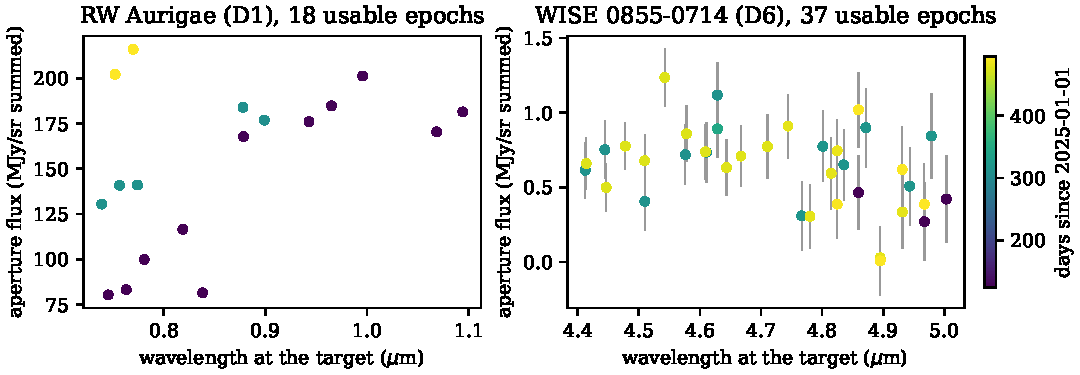
\includegraphics[width=\linewidth]{figures/spectra.pdf}
\caption{Aperture flux against wavelength at the target for every usable epoch, coloured by date. Real data.}
\label{fig:spec}
\end{figure}

\paragraph{E. Speed.} With cutouts cached, one target takes 49--60\,s, including the live archive query and all
pair comparisons; the first analysis of a new target also downloads 45--58 cutouts and takes 1--4 minutes. After
the analysis the app's requests are fast: epoch and pair images $p_{50}=30$\,ms, $p_{95}=42$\,ms; the evidence file
$p_{50}=14$\,ms, $p_{95}=20$\,ms (90 requests each, one laptop CPU).

\section{How robust are the conclusions?}\label{sec:rob}
After the results above were fixed, we audited the measurement for nine possible problems and repeated it under
other reasonable analysis choices (code in \texttt{robustness.py}, results in
\texttt{robustness.json}). The production numbers did not move: the same pairs, ratios and significances as the
published evidence files, to the last digit.
\begin{itemize}\setlength\itemsep{1pt}
\item \textbf{Bad pixels and missing sky.} The photometry used to fall back silently to a sky of zero when the annulus
was empty, and did not refuse a flagged pixel inside the aperture. Neither happened in our data, but both now return
no flux and the pair is refused (two new tests).
\item \textbf{Errors after reprojection.} A simulation of pure noise rotated by $37^\circ$ and shifted onto another
grid, as in our comparison, gives a scatter of the aperture flux of 0.99 times the predicted error, so aperture
errors are right. Single pixels were not: the per-pixel significance map used $\sum w\sigma^2$ instead of
$\sum w^2\sigma^2$ and its scatter was 0.56 of the prediction. With the correction it is 0.94. This changes only the
significance map, not any result. The excess spread for RW~Aur in the null test is therefore not caused by
reprojection; we do not yet know its origin.
\item \textbf{PSF width.} A star whose FWHM grows from 1.5 to 2.0\,px loses 7\% inside our 2\,px aperture (0.4\% at
3\,px). Within each of our pairs the header FWHM is the same (1.22\,px for RW~Aur, 1.47\,px for WISE~0855).
\item \textbf{Wavelength.} Our pairs differ by 0.5--6.8\,nm, against half-channel limits of 8.5--11\,nm, which the
band-centre accuracy of \textcite{hui2026} supports. With the rule tightened to 0.25 or loosened to 0.75 of a channel
(2, 8, 12 RW~Aur pairs; 11, 27, 38 WISE~0855 pairs) every conclusion still holds.
\item \textbf{Calibration between epochs.} Instead of one control star we also use every clean, isolated field star at
$S/N\ge10$ in the cutout. Our $29\times29$\,px cutouts hold only 0--2 such stars, so this ensemble is small. Its scatter
gives a calibration floor of 12.5\% for RW~Aur. Added to the formal errors, the RW~Aur significances become 0.7--12.4$\sigma$
instead of up to $175\sigma$, and the target still changes by 1.5--3.0 times relative to the field stars.
\item \textbf{Many tests.} With 8 (RW~Aur) or 27 (WISE~0855) pairs, the chance of at least one false $5\sigma$ event
is $5\times10^{-6}$ or $1.5\times10^{-5}$; keeping the single-test rate would need $5.4\sigma$ or $5.6\sigma$.
The RW~Aur detection passes both.
\end{itemize}

\textbf{Stability.} Each claim was rechecked with aperture radii 1.5--3\,px, three sky annuli, the flags as given or
grown by one pixel, with and without ensemble calibration, dropping each pair in turn, with the calibration floor
and with the three wavelength rules. We call a claim \emph{robust} if it holds in every check, \emph{sensitive} if in
at least half and \emph{inconclusive} otherwise. This is a fixed rule, not a probability.
\begin{table}[h]\centering\small
\begin{tabular}{lcc}\toprule
Claim & Holds & Label\\\midrule
RW~Aur brightened $\ge\times1.5$ at $\ge5\sigma$ in some pair & 24/24 & robust\\
RW~Aur brighter in \emph{every} pair, one at $\ge5\sigma$ & 18/24 & sensitive\\
WISE~0855: no pair changes by $\ge5\sigma$ & 34/34 & robust\\
Barnard's Star & -- & refused (saturated)\\\bottomrule
\end{tabular}
\caption{Stability of each claim. The second RW~Aur claim fails only with a 1.5\,px aperture, where one pair
(ratio 1.09) falls just below 1. For WISE~0855 only 4 settings keep every pair measurable.}
\label{tab:rob}
\end{table}
The app shows the same checks as a heatmap for each preset. The full analysis of the three targets from cached data
takes 29\,s with 215\,MB of memory.

\textbf{What we did not do, and why.} The SPHEREx images carry an empirical PSF per detector zone (HDU \texttt{EPSF}),
so forced PSF photometry is possible; Section~\ref{sec:epsf} tests it as a second measurement. Proper image
subtraction \parencite{zackay2016} we did not try. A real zero-point fit across epochs \parencite[ubercalibration,][]{padmanabhan2008} needs many stars per
image and larger cutouts. Learned real/bogus classifiers \parencite{duev2019,mahabal2019} and conformal $p$-values
\parencite{bates2023} need a large labelled or null set that three targets do not provide.

\section{Independent ePSF-based photometric verification}\label{sec:epsf}
\textbf{Status: IMPLEMENTED and EXPERIMENTAL.} Nothing in Sections~\ref{sec:val}--\ref{sec:rob} uses it; it lives on a
separate branch (\texttt{psf\_photometry.py}, \texttt{reproduce\_epsf.py}, results in \texttt{epsf\_check.json}).

\textbf{Method.} Each cutout carries the SPHEREx effective PSF as a $21\times21$ grid of zones, each a $33\times33$ table
oversampled $\times5$. We take the zone nearest the star in parent-detector pixels (cutout pixel $+1-$\texttt{CRPIX1A},
as in the IRSA tutorial), record its SHA-256, and fit amplitude $\times$ ePSF $+$ constant background to the $9\times9$
native pixels by weighted least squares ($1/\mathrm{VARIANCE}$). Nothing is reprojected. A flagged pixel within 1.5\,px
of the star refuses the fit, as in the aperture photometry. For stars with S/N $\ge20$ the position may move by up to
1\,px; fainter stars stay at the WCS position. When $\chi^2_\nu>1$ the error is scaled by $\sqrt{\chi^2_\nu}$.
The ePSF as stored fits RW~Aur better than the same table flipped in $x$ in 4 of 5 epochs tried.

\textbf{RW Aur (fitted as one unresolved source; the two stars are 1.4$''$ apart).} All 8 pairs are
\emph{compatible} under the rule fixed beforehand ($|z|<3$, discrepant at $|z|\ge5$, $z$ the difference of the
log-ratios over their combined error): the ePSF ratios are within 0--2\% of the aperture ratios ($|z|\le1.3$),
all 8 pairs are brighter later and every pair is $\ge5\sigma$ with the ePSF alone ($10$--$66\sigma$, lower than the
aperture values because of the $\chi^2$ scaling). The $r=2$\,px aperture holds a steady 96--98\% of the ePSF flux.
The fit is not perfect: $\chi^2_\nu=4$--18 at S/N $\approx300$, with residuals at the core
(Fig.~\ref{fig:epsf}), and the best position is 0.12--0.21\,px from the WCS position in every epoch.
Both methods read the same photons, so their errors could be correlated. We measured this with SIMULATED stars
injected into the real WISE~0855 cutouts: the scatter of $\ln(F_\mathrm{ap}/F_\mathrm{ePSF})$ is 0.95 and 0.99 times
the quadrature error at S/N 10 and 50 (weak correlation), and 1.72 times at S/N 200, where an extra scatter appears,
probably from the star's position inside the pixel. Dividing $z$ by the strictest factor (0.95) leaves all 8 RW~Aur
pairs compatible ($|z|\le1.37$). The injected stars follow the ePSF exactly, so this test does not include the
model error seen in the real residuals.

\textbf{WISE 0855.} Fluxes are below S/N~5, so ratios are not compared (all 27 pairs \emph{inconclusive} by the rule).
The published claim is still checked: no pair reaches $5\sigma$ with the ePSF either (largest $3.1\sigma$; aperture
$1.9\sigma$). \textbf{Barnard's Star} is not fitted: no epoch is usable.

\textbf{SIMULATED tests on real backgrounds.} At 104 blank spots in the 37 usable WISE~0855 cutouts the fit with no star
gives amplitude/error with standard deviation 1.07 and no $|z|\ge3$, so the errors are about right and there were no
false detections. Stars injected at S/N~10 are recovered exactly on top of the blank fit (the model is linear); a
0.3\,px position error loses 7\% of the flux, which is why bright stars fit their position.

\textbf{Combined label (fixed rule).} SUPPORTED VARIABILITY needs a robust aperture claim of change, every pair
compatible and $\ge5\sigma$ with the ePSF; LIKELY ARTIFACT a $\ge5\sigma$ aperture change the ePSF contradicts;
INSUFFICIENT DATA no usable epoch; INCONCLUSIVE anything else. RW~Aur: \textbf{supported variability}. WISE~0855:
\textbf{inconclusive} (no change seen, at S/N too low to prove constancy). Barnard's Star: \textbf{insufficient data}.
These are labels from a rule, not probabilities.

\textbf{Not validated / future work.} Only one ePSF per epoch (no PSF variation inside the $9\times9$ box), a constant
background, no wavelength dependence within the channel; the correlation test above uses stars that match the ePSF exactly.

\begin{figure}[h]\centering
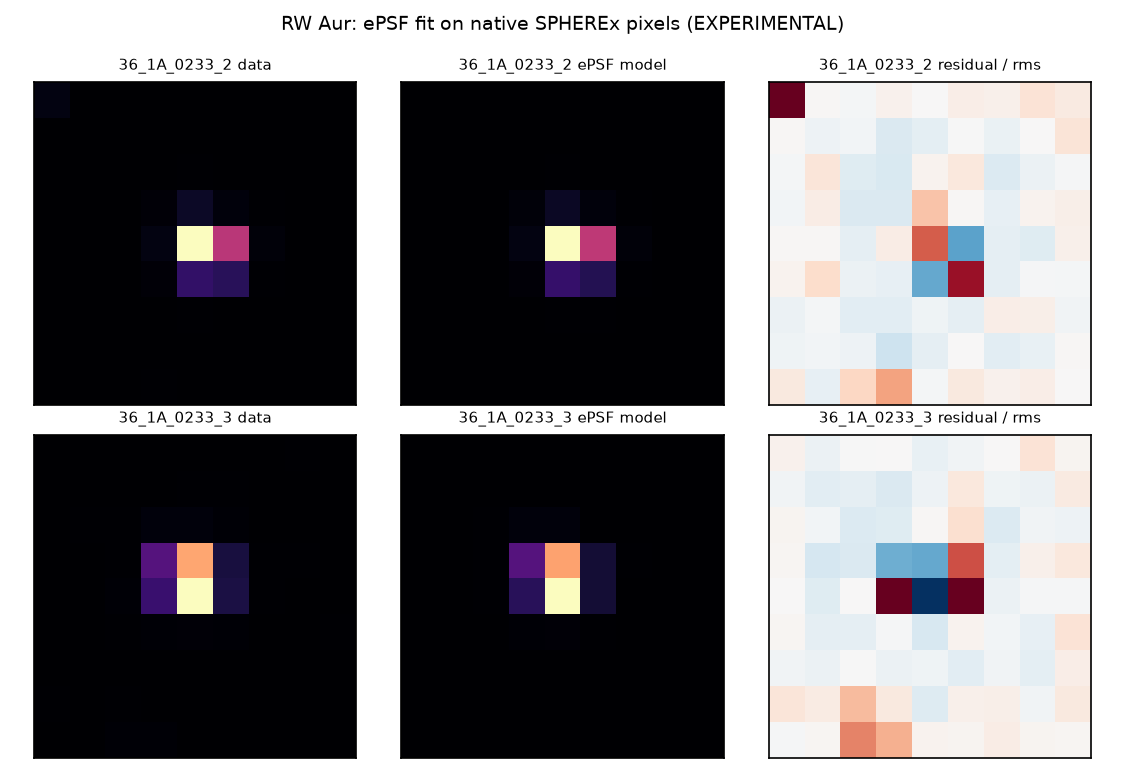
\includegraphics[width=0.85\linewidth]{figures/epsf_residuals.png}
\caption{ePSF fit to two RW~Aur epochs on the native pixels (EXPERIMENTAL): data, model, residual/rms.}\label{fig:epsf}
\end{figure}

\section{Limitations}
\begin{itemize}\setlength\itemsep{1pt}
\item Fluxes are relative (aperture sums of surface brightness). They are adequate for ratios at matched wavelength
but are not calibrated flux densities.
\item The SPHEREx PSF is undersampled; aperture photometry after bilinear reprojection carries a systematic error that
the formal $\sigma$ does not include. The control star bounds it to roughly 15\% and the field stars to 12.5\%
(Section~\ref{sec:rob}). The 175$\sigma$ figure is therefore a formal value; the size of the change ($\times2.5$) is
the robust result.
\item The result uses one control star, and not every pair has one; the field-star check has only 0--2 stars per cutout. Target positions are approximate priors checked
against catalogues only after the analysis. SPHEREx pixels are $6.15''$, so the RW~Aur measurement is of both
components of the binary together, not of one star.
\item Injection-recovery inserts stars after reprojection and without their own photon noise; it measures the
detection threshold of the comparison step, not of the full pipeline.
\item We did not build a machine-learning ranker or a Bayesian model of candidates: with three targets and no
labelled set of real and false changes there is nothing to train or test such a model on honestly. A simple
$5\sigma$ threshold with a control star is the baseline any such model would have to beat.
\item The brightening of RW Aur is consistent with its known variability. It is a measurement from SPHEREx data, not a
discovery, and should be confirmed independently, for example against other surveys.
\end{itemize}

\section{Conclusions}
HIPPARCHUS turns ``compare these two SPHEREx images'' into a checked procedure: it matches wavelength across LVF
epochs, removes zodiacal light, honours pipeline flags, quantifies uncertainty, checks calibration on a control star,
and refuses when the data cannot support an answer. On real data it measures a strong, self-consistent brightening of
RW~Aur, refuses saturated Barnard's Star, and reports no detectable change for faint WISE~0855.

\section{Reproducibility}
\sloppy % long file paths below would otherwise run into the margin
Code: repository \texttt{HIPPARCHUS} (MIT licence), evidence produced at commit \texttt{ffdb565}, validation at \texttt{fe7cba1}, catalogue match at \texttt{aa79a9e}. Run
\texttt{python backend/scripts/reproduce\_evidence.py} to rebuild \texttt{submission/evidence/*.json} (identifiers,
archive query URLs with SHA-256 of each answer, cutout URLs and checksums, settings, software versions, outputs),
\texttt{python backend/scripts/reproduce\_validation.py} for the null test, injection-recovery, spectra, evidence
graphs and timings, \texttt{python backend/scripts/reproduce\_catalogs.py} for the catalogue match,
\texttt{python backend/scripts/reproduce\_robustness.py} for the audit and stability checks, \texttt{python backend/scripts/reproduce\_epsf.py} for the experimental ePSF check (12\,s, 170\,MB), then \texttt{report/reproduce\_report.sh} to rebuild the figures and this PDF.

\section*{Use of AI tools}
AI tools were used mainly for the graphics: the logos, which carry a visible ``AI-generated'' watermark, and
putting together the demo video. They were also used to cross-check the NASA/IRSA dataset references and as a coding
assistant. All code was run and tested by the author. The data, measurements and results all come from real SPHEREx
images; nothing in the Results section or the evidence files was generated by AI.

\section*{Acknowledgments}
This work is based on data from SPHEREx, a NASA mission, obtained from the NASA/IPAC Infrared Science Archive, which is
funded by NASA and operated by the California Institute of Technology. It uses Astropy
\parencite{astropy2013,astropy2018,astropy2022}, NumPy \parencite{numpy2020}, SciPy \parencite{scipy2020}, Matplotlib
\parencite{matplotlib2007}, and the \texttt{reproject} package of the Astropy project.

\printbibliography
\end{document}
